\section{第三章\ 英雄集结：让世界容纳千军万马} 
% 谢先衍 接第二章的尾 把问题重述一遍 然后解释一下

第二章完成了从单机思维到在线思维的范式迁移：我们建立了以权威服务器为核心的CS架构，通过连接管理、状态仲裁与世界同步三大模块，实现了双人对战的稳定运行。这一原型验证了"服务器作为唯一真相源"的正确性，也为后续扩展奠定了可验证的基线。

然而，当我们尝试将这个双人原型扩展为"多人同图"时，会立即遭遇新的系统瓶颈。这不是玩法设计的问题，而是计算资源组织方式的根本性挑战。当地图中同时存在数十乃至上百名玩家时，每秒产生的状态更新事件、位置同步请求、战斗判定计算将呈指数级增长。如果服务器仍然采用"顺序处理每个请求"的朴素模式，响应延迟会迅速恶化，最终导致玩家体验崩塌。

本章的核心命题是：在单机资源边界内，如何通过并发模型与性能优化，将服务器从"能跑双人"提升到"稳定承载多人同图"。这一阶段对应云计算能力曲线中的纵向优化阶段——在进行分布式横向扩展之前，必须先把单机潜力压榨到极致，建立可观测的性能基线，从而判断何时应该继续优化、何时必须转向分布式架构。我们将从并发模型的建立、共享数据的安全保护，以及资源池化与数据分层三个维度，系统性地解决单机服务器在高并发场景下的核心约束。

% \subsection{万人集结：并发的奥秘} 
\subsection{万人集结：并发的系统必然性}
% 什么是并发
% 协程需要介绍一下 与线程 进程的区别 并发在goroutine中的体现 -> 协程
% 
% \paragraph{本节目标}  理解并发本质，掌握 Go 的 goroutine+Channel 逻辑。

\subsubsection{多人同图下的系统瓶颈}

在第二章的双人原型中，服务器的处理逻辑相对简单：接收玩家A的移动请求，验证其合法性，更新状态后广播给玩家B；接着以相同流程处理玩家B的请求。由于只有两个连接、有限的事件密度，顺序执行模式完全可以满足实时性要求。然而，当我们将场景扩展到"50人同图"时，系统负载特征发生质变，暴露出顺序执行模型在高并发场景下的四大核心瓶颈。

\begin{figure}[H]
    \centering
    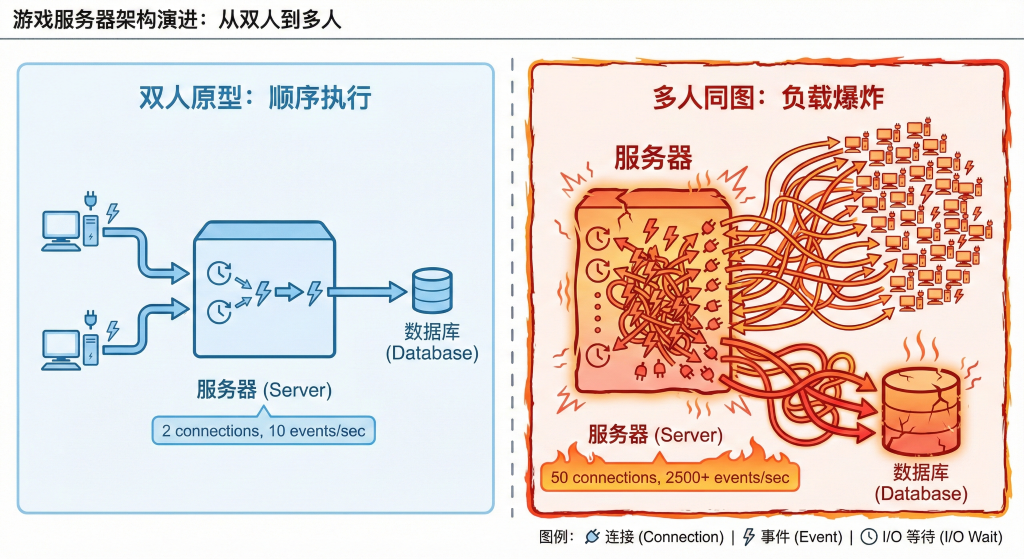
\includegraphics[width=1.0\linewidth]{figures/sec3/image3-1.png}
    \caption{从双人原型到多人同图的系统负载变化：连接数、事件密度和I/O等待的指数级增长}
    \label{fig:concurrent-load}
\end{figure}

第一个瓶颈是连接规模的爆炸性增长。系统需要维护的WebSocket长连接数从2个增长到50个，而每个连接都需要独立的读写缓冲区、心跳检测机制与超时管理逻辑。如果采用传统的"一个操作系统线程处理一个连接"模型，每个线程需要预分配约1到8MB的栈空间，50个连接就可能消耗数百MB内存。更严重的是，操作系统线程的创建和销毁涉及系统调用，上下文切换需要保存和恢复完整的CPU寄存器状态，这些开销在高频场景下会成为显著的性能拖累。当连接数增长到数百、数千时，传统线程模型将因内存耗尽和调度开销过大而崩溃。

第二个瓶颈是事件密度的指数级放大。假设每名玩家平均每秒发送5次操作（包括移动、攻击、技能释放等），服务器就需要处理250次每秒的输入事件。但这只是输入侧的负载，输出侧的压力更为严峻。每次状态变更都需要广播给视野内的其他玩家，假设平均每人视野内有10名玩家，则每秒需要发送2500次状态同步消息。这种广播放大效应使得网络带宽消耗和消息序列化开销呈平方级增长。在顺序执行模型中，处理这些事件的总时间是所有单次操作时间的简单累加，当事件密度超过处理能力上限时，消息队列会迅速积压，响应延迟从毫秒级恶化到秒级。

第三个瓶颈是I/O等待时间的全局传播。在单机服务器中，许多操作都涉及I/O等待：从Redis读取玩家位置需要等待网络往返，从PostgreSQL查询装备信息需要等待磁盘读取，向客户端发送消息需要等待TCP缓冲区就绪。在顺序执行模型中，主线程在等待玩家A的数据库响应时会完全阻塞，无法处理其他玩家的请求。这意味着一个玩家的数据库延迟会传播到所有其他玩家，造成全局性的响应延迟增长。即使系统配备了高性能CPU和大容量内存，这些计算资源也会因为I/O等待而长时间处于空闲状态，资源利用率极低。

第四个瓶颈是共享资源的并发访问冲突。当多个玩家几乎同时操作同一资源（如拾取地图上唯一的宝箱、攻击同一个Boss、占领同一个据点）时，系统必须确保操作的原子性和结果的确定性。在单线程模型中，这个问题被天然规避了——所有操作按照到达顺序依次执行，不存在并发冲突。但一旦引入并发处理，如果没有合理的同步机制，就可能出现"两人都认为自己拾取成功"的数据竞争，破坏游戏规则的公平性和确定性。这类问题的根源在于检查和修改操作之间存在时间窗口，多个执行流可能同时通过检查条件并执行修改操作。

这四大瓶颈不是网络游戏特有的现象，而是所有高并发在线服务在单机阶段必然遭遇的通用约束。无论是即时通讯系统、金融交易平台，还是协同办公应用，只要系统需要同时服务大量并发用户，就会面临相同的资源组织挑战：多路连接的高效管理、高频事件的吞吐压力、I/O密集操作的延迟控制，以及共享状态的并发安全。并发编程正是应对这类挑战的系统级解决方案，其核心目标不是"让单个任务跑得更快"，而是通过合理的任务拆解与调度，在给定的硬件资源约束下，最大化系统的整体吞吐量并维持可接受的响应延迟。

并发（Concurrency）在系统设计中，是指将一个复杂任务拆解为多个可独立推进的执行单元，使它们能够在逻辑上同时进行，从而充分利用等待时间、提升整体吞吐量并保持响应及时性的任务组织方式。对于游戏服务器而言，并发意味着不同玩家的请求可以被并行处理，玩家A的数据库查询不会阻塞玩家B的移动验证；I/O等待时间可以被有效利用，当等待Redis响应时，CPU可以去处理其他玩家的逻辑计算；状态更新可以被异步广播，主逻辑线程完成裁决后立即返回，由独立的通知协程负责消息分发。需要强调的是，并发不是为了"让程序跑得更快"的性能调优技巧，而是在单机资源约束下维持系统可用性的基础组织方式。当负载超过顺序执行模型的承载上限时，不引入并发，系统就会因响应超时、连接积压而实质性不可用。

\subsubsection{Goroutine：轻量级并发的工程实现}

确立了并发作为任务组织方式的必要性后，下一个问题是：如何在工程上实现高效的并发？传统操作系统线程模型虽然可用，但在高并发场景下存在明显的资源成本问题。每个操作系统线程需要预分配约1到8MB的栈空间用于存储函数调用链和局部变量，创建线程时需要通过系统调用向内核申请资源，销毁线程时需要释放相关的内核数据结构。在高频连接场景下，如果为每个新连接创建一个线程，又在连接关闭时销毁该线程，这种频繁的创建和销毁操作会产生显著的资源抖动，大量CPU时间被消耗在系统调用和上下文切换上，而非实际的业务逻辑处理。此外，线程切换需要保存和恢复完整的CPU上下文，包括寄存器、程序计数器、栈指针等状态信息，每次切换的开销在微秒级别。对于I/O密集型的游戏服务器，如果有数千个线程频繁进入和退出阻塞状态，操作系统调度器会将大量时间用于上下文切换而非实际计算。更严重的是，受内存与调度器压力的限制，单机能稳定运行的线程数通常在数百到数千量级，难以支撑万级连接的并发场景。

\begin{figure}[H]
    \centering
    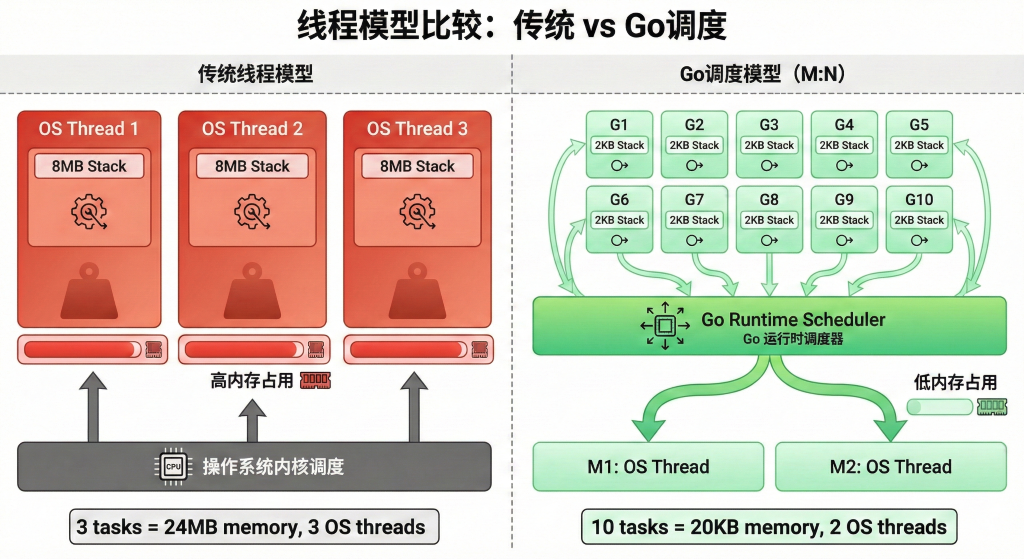
\includegraphics[width=1.0\linewidth]{figures/sec3/image3-2.png}
    \caption{传统操作系统线程模型与Go的M:N调度模型对比：Goroutine通过用户态调度实现高并发低开销}
    \label{fig:goroutine-model}
\end{figure}

Go语言通过Goroutine提供了一种更轻量的并发原语来解决传统线程模型的性能瓶颈。Goroutine是Go运行时在用户态管理的协程（coroutine），其核心设计理念是将并发执行单元的创建和调度从操作系统内核上移到语言运行时层面，从而获得更细粒度的控制能力和更低的资源开销。Goroutine的优势体现在多个维度。首先是极低的内存占用，每个Goroutine的初始栈空间仅2KB，相比操作系统线程的1到8MB栈空间，内存效率提升了数百倍。更重要的是，Goroutine的栈空间可以根据实际需要动态增长和收缩，避免了预分配大块内存导致的浪费。这使得在单机上同时运行数万甚至数十万个Goroutine成为可能，为"One Goroutine Per Connection"的架构模式提供了资源保障。

其次是高效的M:N调度模型。Go运行时维护少量操作系统线程（记为M），在其上调度大量Goroutine（记为N），形成M:N的多对多映射关系。这种设计的核心价值在于解耦了逻辑并发度和物理并行度。当某个Goroutine因等待I/O操作（如网络读取、数据库查询）而阻塞时，Go调度器会自动将其挂起并将该操作系统线程分配给其他可运行的Goroutine继续执行，而不是让整个线程进入阻塞状态。这种协作式调度机制使得I/O等待不再导致线程资源的浪费，CPU可以持续处理就绪的任务，显著提升了资源利用率。对于I/O密集型的游戏服务器，这意味着即使有数千个Goroutine在等待网络响应或数据库查询，实际占用的操作系统线程数仍然可以维持在几十个到几百个的合理范围内，避免了线程爆炸问题。

最后是简化的编程模型。开发者只需用\texttt{go}关键字启动并发任务，无需手动管理线程的创建、销毁、同步等底层细节，Go运行时负责所有调度策略和资源管理。这种抽象大幅降低了并发编程的心智负担，使得并发逻辑的表达更加接近业务语义。在游戏服务器的场景下，可以直接用"为每个玩家连接启动一个Goroutine"的自然表达来组织代码，而不需要考虑线程池大小、任务队列长度等底层实现细节。

为了直观展示Goroutine带来的性能提升，我们通过对比实验来量化顺序执行与并发执行的差异。假设需要为3名玩家分别执行一个耗时2秒的数据加载操作（如从数据库读取装备信息并进行复杂计算）。在顺序执行版本中，服务器必须等待玩家A的操作完全完成后，才能开始处理玩家B的请求，玩家C则需要等待前两个请求全部完成。这种串行处理模式导致总执行时间是单次操作时间的线性累加，三名玩家的总耗时达到6秒。对于实时游戏，6秒的等待意味着玩家C会看到明显的卡顿，严重影响用户体验。

% \begin{tcolorbox}[title=顺序执行模式的性能瓶颈]
% \begin{verbatim}
% func handlePlayer(playerID string) {
%     fmt.Printf("开始处理玩家 %s...\n", playerID)
%     time.Sleep(2 * time.Second) // 模拟I/O等待
%     fmt.Printf("玩家 %s 处理完成\n", playerID)
% }

% func main() {
%     startTime := time.Now()
%     // 顺序处理3名玩家
%     handlePlayer("A")
%     handlePlayer("B")
%     handlePlayer("C")
%     fmt.Printf("总耗时: %v\n", time.Since(startTime))
% }
% // 输出：总耗时约6秒，玩家C需要等待4秒才开始被处理
% \end{verbatim}
% \end{tcolorbox}

\begin{tcolorbox}[title=顺序执行模式的性能瓶颈]
\begin{lstlisting}[style=codeblock, language=go]
func handlePlayer(playerID string) {
    fmt.Printf("处理玩家 %s\n", playerID)
    time.Sleep(2 * time.Second) // 模拟数据库查询等I/O操作
}

func main() {
    handlePlayer("A")
    handlePlayer("B")
    handlePlayer("C")
    // 总耗时约6秒：每个玩家必须等待前一个处理完毕
}
\end{lstlisting}
\end{tcolorbox}

而通过\texttt{go}关键字启动Goroutine，三个处理任务可以并发执行，总耗时降低到单次操作的时间。在这个模式下，三个Goroutine由Go调度器分配到可用的操作系统线程上并发执行。如果服务器配备多核处理器，这些Goroutine可以实现真正的并行计算。即使在单核处理器上，由于操作主要是I/O等待而非CPU计算，调度器也可以在等待期间切换到其他Goroutine，充分利用等待时间。更重要的是，这种模式可以无缝扩展到50人、100人，只要单机CPU和内存资源充足，就能维持相近的响应延迟。

\begin{tcolorbox}[title=Goroutine并发模式的性能提升]
\begin{lstlisting}[style=codeblock, language=go]
func main() {
    var wg sync.WaitGroup
    players := []string{"A", "B", "C"}
    
    for _, player := range players {
        wg.Add(1)
        go func(id string) {
            defer wg.Done()
            handlePlayer(id)
        }(player)
    }
    
    wg.Wait()
    // 总耗时约2秒：三个玩家并发处理
}
\end{lstlisting}
\end{tcolorbox}

表\ref{tab:goroutine-performance}展示了顺序执行与并发执行在不同玩家规模下的性能对比。可以看到，当玩家数从3人增长到1000人时，顺序执行的总耗时呈线性增长，而并发执行的耗时基本保持稳定。这种差异在大规模场景下尤为显著，性能提升可达数百倍。

\begin{table}[h]
\centering
\caption{顺序执行与Goroutine并发的性能对比}
\label{tab:goroutine-performance}
\begin{tabular}{lccc}
\hline
\textbf{处理模式} & \textbf{3个玩家} & \textbf{1000个玩家} & \textbf{性能提升比} \\
\hline
顺序执行（串行） & 6秒 & 约2000秒（33分钟） & --- \\
Goroutine并发 & 2秒 & 2--3秒 & 约600--1000倍 \\
\hline
\end{tabular}
\end{table}

在实际的游戏服务器架构中，存在两种典型的Goroutine组织模式。One Goroutine Per Connection模式为每个WebSocket连接分配一个独立的Goroutine，负责该连接从建立到断开的完整生命周期，包括读取客户端消息、解析协议、执行业务逻辑、发送响应等操作。这种模式的优势在于连接的所有状态和上下文都封装在一个Goroutine内部，逻辑清晰且易于管理。One Goroutine Per Request模式则更进一步，即使在同一连接内，也可以为每个独立的业务请求（如发起战斗、查询背包、交易物品）启动临时Goroutine，任务完成后由Go运行时自动回收资源。这种模式适合请求处理时间差异较大的场景，可以避免慢请求阻塞连接上的其他快速请求。在实际工程中，这两种模式往往结合使用，连接层采用Per Connection模式维护长连接状态，业务层根据操作复杂度选择性地使用Per Request模式。

需要注意的是，Goroutine虽然轻量，但并非零成本。每个Goroutine仍然需要占用一定的内存空间和调度器资源，大量创建和销毁仍会给调度器和垃圾回收器带来压力。因此在后续章节中，我们会讨论对象池等优化手段来缓解这些开销。但总体而言，Goroutine提供的轻量级并发能力，为构建高并发游戏服务器奠定了坚实的资源基础，使得"每连接一协程"的架构模式在资源消耗和开发效率之间取得了理想的平衡。

% \subsubsection{Channel：消息沟通取代共享内存}

% \subsubsection{Channel：Goroutine 之间的通信机制}

\subsubsection{Channel：事件驱动的协程通信机制}

引入Goroutine解决了"如何高效并发"的问题，但随之而来的是新的挑战：并发的Goroutine之间如何安全地交换数据和协调执行顺序？传统多线程编程中，通常通过共享内存加锁的方式实现通信——多个线程直接访问同一块内存区域，通过互斥锁保护临界区来避免数据竞争。这种模式虽然直观，但容易引发死锁、优先级反转、数据竞争等难以调试的并发Bug，尤其在复杂的业务逻辑中，锁的获取顺序稍有不慎就可能导致系统陷入僵局。

Go语言倡导的并发哲学是："不要通过共享内存来通信，而应该通过通信来共享内存"。这一理念强调将数据的所有权在Goroutine之间显式传递，而非让多个Goroutine同时持有对同一数据的引用。这种设计哲学的载体就是Channel——Go提供的一种类型安全的消息队列，专门用于Goroutine之间传递数据。Channel的本质是一个先进先出的队列，配合发送和接收操作的阻塞语义，可以自然地实现Goroutine之间的同步和协调。

Channel分为无缓冲通道和有缓冲通道两种类型，两者在同步语义上有本质区别。无缓冲通道要求发送和接收操作必须同时就绪才能完成，具有强同步语义。当一个Goroutine向无缓冲通道发送数据时，它会阻塞等待直到另一个Goroutine从该通道接收数据，这种"握手"机制可以精确控制Goroutine之间的执行顺序。有缓冲通道则允许在缓冲区未满时异步发送数据，缓冲区未空时异步接收数据。发送方只有在缓冲区满时才会阻塞，接收方只有在缓冲区空时才会阻塞。有缓冲通道的价值在于解耦生产者和消费者的处理速度，允许短时间内的速率差异，避免生产者因消费者处理较慢而被频繁阻塞。

在游戏服务器开发中，Channel的典型应用场景是将玩家操作事件异步分发给处理协程，实现网络I/O层和业务逻辑层的解耦。考虑这样的架构设计：每个玩家连接对应一个读取Goroutine（负责从WebSocket读取消息并反序列化）和一个处理Goroutine（负责执行业务逻辑如移动验证、战斗计算、状态更新）。两者通过一个有缓冲的Channel连接，读取Goroutine将解析后的消息对象发送到Channel，处理Goroutine从Channel接收消息并执行相应逻辑。

\begin{tcolorbox}[title=使用Channel实现消息异步处理]
\begin{lstlisting}[style=codeblock, language=go]
type PlayerMessage struct {
    PlayerID string
    Action   string
    Data     interface{}
}

func handlePlayerConnection(playerID string) {
    msgChan := make(chan PlayerMessage, 100)
    
    go func() {
        for msg := range msgChan {
            processMessage(msg)
        }
    }()
    
    // 接收并发送消息到channel
    for i := 0; i < 5; i++ {
        msgChan <- PlayerMessage{
            PlayerID: playerID,
            Action:   "move",
            Data:     fmt.Sprintf("position:%d", i),
        }
    }
    
    close(msgChan)
}
\end{lstlisting}
\end{tcolorbox}

这种设计带来了多个层面的架构优势。首先是读写解耦，网络I/O和业务逻辑完全分离为独立的执行流。读取Goroutine专注于高效地从网络套接字读取字节流并进行协议解析，不需要等待业务逻辑执行完成就可以继续接收下一条消息。即使业务处理较慢（如涉及复杂的战斗计算或数据库查询），也不会阻塞消息接收，保证了系统的响应性。其次是流量控制，有缓冲的Channel可以平滑瞬时流量峰值。当玩家在短时间内连续发送多条操作指令时（如快速点击技能按钮），这些消息会被暂存在Channel的缓冲区中，处理Goroutine可以按照自己的节奏从缓冲区取出消息依次处理，避免了生产者速率过快导致的消费者过载问题。最后是优雅关闭，通过\texttt{close(channel)}可以通知所有接收方停止等待。当连接断开时，读取Goroutine关闭消息Channel，处理Goroutine在处理完缓冲区中的剩余消息后会感知到通道已关闭，自动退出循环并进行资源清理。这种基于通道关闭的退出机制比通过共享标志位检查更加简洁和可靠。

\begin{figure}[H]
    \centering
    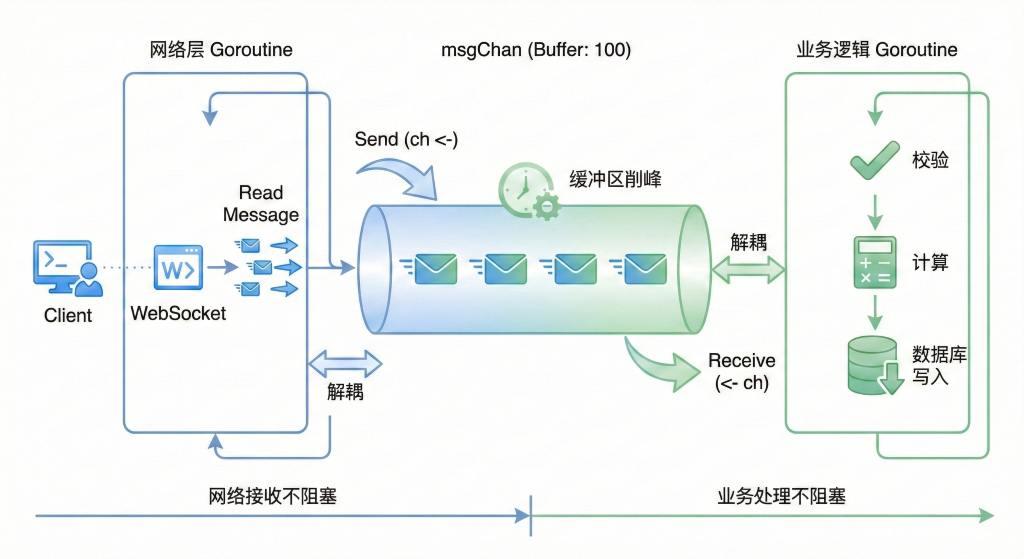
\includegraphics[width=1\linewidth]{figures/sec3/image3-3.png}
    \caption{基于Channel的消息异步处理架构：网络I/O与业务逻辑解耦，实现流量削峰和非阻塞处理}
    \label{fig:channel-async}
\end{figure}

当需要同时监听多个Channel或处理超时时，Go提供了\texttt{select}语句进行多路复用。\texttt{select}语句在语法上类似于\texttt{switch}，但每个\texttt{case}分支对应一个通道操作（发送或接收）。\texttt{select}会阻塞等待直到至少有一个\texttt{case}分支的通道操作可以执行，如果多个\texttt{case}同时就绪，则随机选择一个执行。这种机制在游戏服务器中可用于实现超时控制和心跳检测。

\begin{tcolorbox}[title=使用Select实现超时控制]
\begin{lstlisting}[style=codeblock, language=go]
func handleWithTimeout(playerID string, msgChan chan PlayerMessage) {
    for {
        select {
        case msg := <-msgChan:
            processMessage(msg)
        case <-time.After(30 * time.Second):
            fmt.Printf("玩家 %s 超时，断开连接\n", playerID)
            return
        }
    }
}
\end{lstlisting}
\end{tcolorbox}

在这个示例中，\texttt{select}语句同时监听两个事件源：消息Channel和超时定时器。如果30秒内\texttt{msgChan}收到新消息，则执行第一个\texttt{case}分支进行正常处理；如果30秒内没有任何消息到达，\texttt{time.After}会向其返回的通道发送一个时间值，触发第二个\texttt{case}分支执行超时处理逻辑。这种模式在游戏服务器中用于实现心跳检测：如果玩家长时间不发送任何消息（包括心跳包），服务器会主动断开连接释放资源，防止僵尸连接占用系统资源。

从系统设计的角度看，Channel提供的是一种事件驱动的并发架构模式，这种模式与Actor模型有异曲同工之处。每个Goroutine可以被视为一个独立的执行单元，它们不直接访问彼此的内存空间，而是通过发送消息来协作完成复杂任务。这种基于消息传递的并发模型天然地降低了数据竞争风险，因为数据的所有权在不同Goroutine之间显式转移，避免了多个执行流同时修改同一数据的情况。更重要的是，这种架构模式为后续的分布式扩展埋下了平滑演进的伏笔。当系统从单机演化为多机时，Goroutine之间的Channel可以被替换为跨网络的RPC调用或消息队列（如Kafka、RabbitMQ），而业务逻辑的组织方式基本保持不变。这种从进程内通信到进程间通信、从单机并发到分布式并发的平滑过渡，正是基于消息传递的并发模型的核心价值所在。

然而，引入Goroutine和Channel后，我们获得了并发处理多人请求的能力，但并发也带来了新的风险。当多个Goroutine需要访问同一份共享数据时，如何保证操作的原子性与结果的确定性？这正是下一节要解决的核心问题——并发环境下的规则可信度保障。


% \paragraph{写作建议}
% \begin{enumerate}
%     \item 要先讲 单线程 的痛点，引出并发作用（同时处理多请求），点出 goroutine（协程） 轻量优势。
%     \item 讲清goroutine和Channel的协作逻辑：
%     \paragraph{}在游戏场景中，单一 goroutine 处理所有玩家请求会导致性能瓶颈，因为玩家的操作请求（如移动、攻击等）是并发产生的。采用多 goroutine 模式，为每个玩家分配独立的 goroutine（如玩家 1 的请求由专属 goroutine 处理），能并行处理不同玩家的操作，大幅提升系统响应速度。
%     \paragraph{} 当多个 goroutine 同时访问和修改共享数据（例如双玩家争抢地图上同一位置资源）时，会出现数据竞争问题，导致游戏状态混乱。通过 Channel 传递数据，可将并发访问限制为顺序执行：数据的生产和消费通过 Channel 进行同步，只有当接收方准备好时，发送方才能传递数据，从而避免多个 goroutine 同时修改同一数据，有效解决数据竞争带来的冲突问题，确保游戏状态的一致性和稳定性。
%     \item 铺垫锁：操作同一资源需加锁，为 3.3 做准备。
% \end{enumerate}

\subsection{混乱中的秩序：“锁"住你的虚拟宝藏}

在上一节中，我们通过Goroutine实现了"每个玩家独立处理"的并发模型，显著提升了系统吞吐量。但并发带来新能力的同时，也引入了新的风险：当多个Goroutine需要访问同一份共享数据时，如何保证操作的原子性与结果的确定性？这不仅仅是编程技巧问题，更是多人在线游戏规则可信度的工程基础。在游戏这种强对抗性的环境中，任何规则的不确定性都会被玩家直接感知并放大为体验问题，甚至引发对系统公平性的质疑。

\subsubsection{当两个玩家同时捡起一把剑}

考虑这样一个典型场景：地图上刷新了一把稀有武器（如传说级屠龙刀），系统中仅存在这唯一的一把。同一时刻，玩家A和玩家B几乎同时触发了拾取操作。从玩家的业务视角看，这是一个简单的"先到先得"规则——谁先完成拾取动作，谁就应该获得该装备，另一名玩家则应该看到"物品已被拾取"的提示。但从系统实现的角度看，这个看似简单的业务规则背后涉及一系列并发操作的正确协调。玩家A的Goroutine首先读取全局的\texttt{hasItem}标志，发现其值为\texttt{true}，判定物品存在，随即开始执行拾取逻辑。几乎在同一时刻，玩家B的Goroutine也读取\texttt{hasItem}标志，同样发现其值为\texttt{true}，也通过了存在性检查并进入拾取流程。随后，两个Goroutine分别将\texttt{hasItem}设为\texttt{false}，并各自在内存中更新了所属玩家的背包数据。从执行结果看，两个玩家的客户端都收到了"拾取成功"的响应，但实际上地图上只有一把武器，这违反了物品唯一性的核心规则。

这种现象在并发编程中被称为竞态条件（Race Condition），其根源在于"检查-修改"这一组合操作不是原子的。在玩家A检查到物品存在与将标志设为\texttt{false}之间，存在一个时间窗口。如果玩家B的检查操作落在这个窗口内，两个Goroutine都会通过检查条件并执行修改操作，导致同一资源被多次获取。这种并发访问冲突不仅破坏了游戏内物品的唯一性约束，还可能引发更严重的连锁问题。如果这把稀有武器是限量发行的活动奖励，复制物品会破坏游戏的经济系统平衡，影响其他正常玩家的游戏体验。如果涉及交易系统，一个物品被多个玩家持有可能导致交易记录混乱，甚至引发玩家之间的纠纷。

竞态条件问题并非游戏服务器特有，而是所有需要保证业务规则只产生唯一结果的并发系统都必须面对的核心挑战。在电商系统中，库存扣减操作必须保证原子性，否则会出现超卖现象——实际库存只有10件商品，但由于并发扣减时多个订单同时通过了库存检查，最终可能生成15个订单。在金融系统中，账户转账操作涉及扣减发送方余额和增加接收方余额两个步骤，如果这两个操作不能原子执行，系统在崩溃或并发冲突时可能出现资金凭空消失或凭空增加的双花问题。在协同编辑系统中，多个用户同时修改文档的同一段落，如果缺乏冲突检测和合并机制，可能出现后提交的修改覆盖先提交修改的数据丢失问题。

对于游戏服务器而言，竞态条件的后果尤为严重，因为它直接体现为玩家可感知的规则失效。两人同时拾取导致物品复制，玩家会质疑游戏的公平性；同时攻击导致伤害计算重复，受害玩家会认为遭遇了Bug或外挂；同时占领据点导致归属混乱，团队战术配合会因系统不可预测性而失去意义。这些问题的本质是：在并发环境下，我们需要一种机制来保证关键的业务规则修改是串行执行的，即使多个Goroutine试图同时操作，也只能有一个成功，其他必须等待或收到明确的失败反馈。这正是互斥锁要解决的核心问题。

\subsubsection{实战：没有锁的混乱现场}

让我们通过代码重现这个问题，更直观地理解竞态条件的危害。在下面的示例中，全局变量\texttt{hasItem}表示地图上是否存在可拾取的物品。\texttt{pickItem}函数模拟玩家拾取逻辑，包括检查物品是否存在、模拟处理延迟（如网络往返或数据库写入）、标记物品已被拾取三个步骤。

\begin{tcolorbox}[title=危险代码：缺乏同步保护的并发访问]
\begin{lstlisting}[style=codeblock, language=go]
var hasItem = true // 全局标志：地图上是否有物品

func pickItem(playerID string) {
    if hasItem { // 步骤1：检查物品是否存在
        time.Sleep(time.Millisecond) // 步骤2：模拟延迟
        hasItem = false // 步骤3：标记已拾取
        fmt.Printf("玩家 %s 成功拾取物品\n", playerID)
    } else {
        fmt.Printf("玩家 %s 拾取失败，物品已被抢走\n", playerID)
    }
}

func main() {
    go pickItem("A") // 玩家A的Goroutine
    go pickItem("B") // 玩家B的Goroutine
    time.Sleep(time.Second) // 等待两个Goroutine执行完毕
}
\end{lstlisting}
\end{tcolorbox}

运行这段代码多次，大概率会看到两名玩家都"成功"拾取了物品，少数情况下才会出现正确的结果（一成功一失败）。问题的关键在于步骤1的检查和步骤3的修改之间存在明显的时间窗口。当玩家A执行到步骤1发现\texttt{hasItem=true}后，在执行步骤2的延迟期间，玩家B也执行了步骤1同样发现为\texttt{true}。结果两者都通过了检查条件，进入拾取分支。即使步骤2的延迟很短（只有1毫秒），在高并发场景下这个窗口仍然足够让多个Goroutine同时通过检查。这种并发访问冲突导致同一件稀有装备被多次获取，破坏了游戏内物品的唯一性约束。从更深层次看，这个问题暴露了一个根本性矛盾：在并发环境下，我们需要的不仅是"每个Goroutine都能独立执行"，更需要"对于某些关键操作，多个Goroutine必须排队等待"。如何在保持并发处理能力的同时，对特定的共享资源访问进行串行化控制，这正是下一小节要解决的问题。

\subsubsection{互斥锁：将规则修改收敛为原子操作}

要解决上述竞态条件问题，核心思路是将"检查-修改"这一组合操作变成不可分割的原子区，保证在同一时刻只有一个Goroutine能够执行这段逻辑。互斥锁（Mutex, Mutual Exclusion Lock）正是实现这一目标的基本同步原语。互斥锁的工作机制类似于一个只能同时被一个人持有的令牌：当一个Goroutine需要访问共享资源时，它首先尝试获取锁（调用\texttt{Lock()}方法）；如果锁当前没有被其他Goroutine持有，则成功获取并进入临界区执行关键操作；如果锁已被其他Goroutine持有，则当前Goroutine进入阻塞等待状态，直到持有锁的Goroutine完成操作并释放锁（调用\texttt{Unlock()}方法）。

在Go中，标准库提供了\texttt{sync.Mutex}类型来实现互斥锁。其设计非常简洁，只提供两个核心方法：\texttt{Lock()}用于获取锁，如果锁不可用则阻塞；\texttt{Unlock()}用于释放锁，允许其他等待的Goroutine获取。需要注意的是，对同一个Mutex多次调用\texttt{Lock()}而不释放会导致死锁，因此推荐使用\texttt{defer}语句确保锁一定会被释放，即使函数因\texttt{return}或\texttt{panic}提前退出也不会遗漏。

\begin{figure}[H]
    \centering
    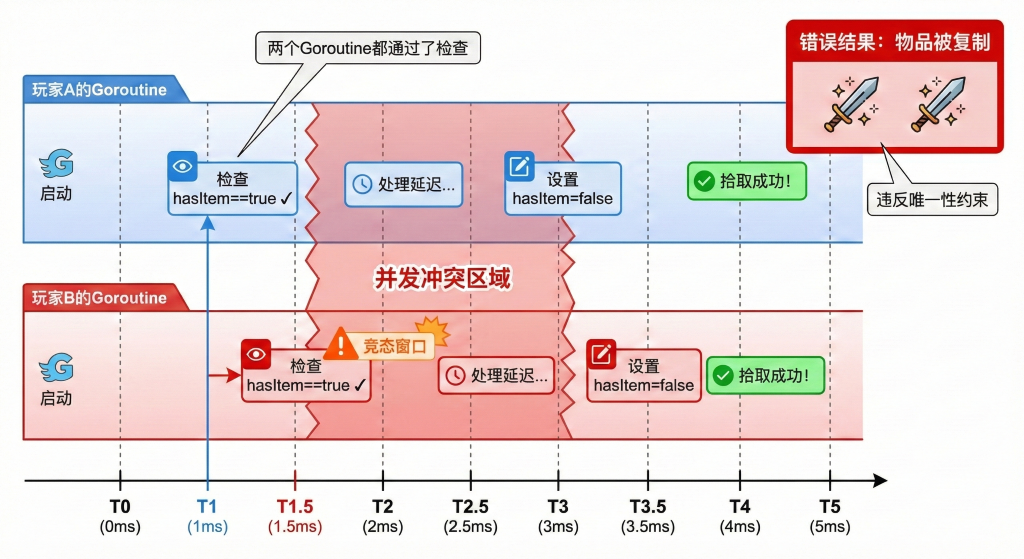
\includegraphics[width=1\linewidth]{figures/sec3/image3-4.png}
    \caption{竞态条件的时序分析：缺乏同步保护导致两个Goroutine同时通过检查并修改共享状态}
    \label{fig:race-condition}
\end{figure}

\subsubsection{实战：加上锁的秩序世界}

现在我们引入\texttt{sync.Mutex}来修复前面的竞态条件问题。在\texttt{pickItemSafe}函数中，通过\texttt{itemLock.Lock()}加锁进入临界区，使用\texttt{defer itemLock.Unlock()}确保无论函数如何退出锁都会被释放。这样，整个"检查-修改"过程被保护在一个原子操作内。

\begin{tcolorbox}[title=安全代码：使用Mutex保护共享资源]
\begin{lstlisting}[style=codeblock, language=go]
var hasItem = true
var itemLock sync.Mutex // 互斥锁

func pickItemSafe(playerID string) {
    itemLock.Lock() // 获取锁，进入临界区
    defer itemLock.Unlock() // 延迟释放锁
    
    if hasItem {
        time.Sleep(time.Millisecond) // 模拟处理延迟
        hasItem = false
        fmt.Printf("玩家 %s 成功拾取物品\n", playerID)
    } else {
        fmt.Printf("玩家 %s 拾取失败，物品已被抢走\n", playerID)
    }
}

func main() {
    go pickItemSafe("A")
    go pickItemSafe("B")
    time.Sleep(time.Second)
}
\end{lstlisting}
\end{tcolorbox}

现在运行结果变为确定性的：玩家A成功拾取物品，玩家B拾取失败。规则恢复了可信度。通过引入互斥锁机制，原本可能并发执行的多个拾取操作被串行化为顺序执行。当玩家A的Goroutine获取锁后，玩家B的Goroutine在尝试获取锁时会被阻塞，直到玩家A完成整个操作并释放锁。这样，无论两个Goroutine的启动时间多么接近，它们对共享资源的访问都会被强制排队，从而保证了在任意时刻只有一个协程能够访问和修改共享数据。\texttt{defer itemLock.Unlock()}的设计是一个重要的工程实践，它利用了Go语言的defer机制，确保即使函数在执行过程中发生\texttt{panic}或通过\texttt{return}提前返回，锁也一定会被释放，避免了其他Goroutine永久阻塞导致的死锁问题。

在使用互斥锁时需要注意几个重要的实现细节和潜在陷阱。首先，Mutex必须通过指针方式传递给函数或作为结构体字段使用。如果按值传递Mutex，会导致锁被复制，每个Goroutine实际上操作的是不同的锁副本，同步保护完全失效。其次，临界区的范围应该尽可能小，只保护必须同步的共享数据访问，而将不需要同步的计算逻辑移出临界区。过大的临界区会导致Goroutine长时间持有锁，降低并发度，使系统性能退化接近单线程。最后，要避免嵌套锁的使用，即在持有锁A的情况下又尝试获取锁B，这很容易因为不同Goroutine的加锁顺序不一致而导致死锁。如果业务逻辑确实需要同时访问多个资源，应该定义明确的加锁顺序并严格遵守。

\subsubsection{锁的粒度：性能与公平的折中设计}

虽然互斥锁解决了并发环境下的正确性问题，但也引入了新的性能成本：串行化。被锁保护的代码块在同一时刻只能被一个Goroutine执行，其他Goroutine必须排队等待。这种串行化执行意味着并发度的降低，如果临界区执行时间较长或访问频率很高，锁竞争会成为系统瓶颈。因此，在实际系统设计中，锁的粒度选择成为一个需要仔细权衡的问题，它本质上是在并发性能和实现复杂度之间寻找平衡点。

\begin{figure}[H]
    \centering
    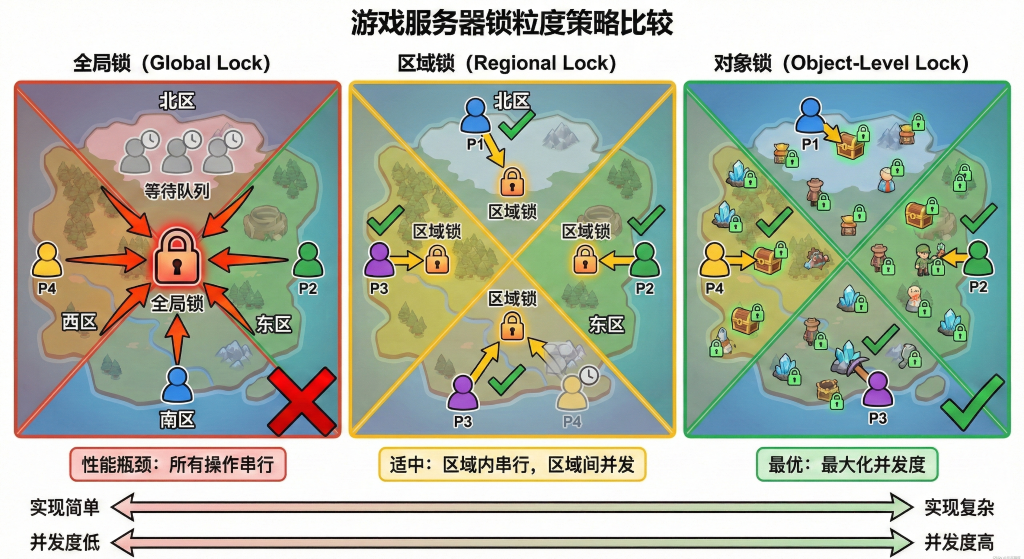
\includegraphics[width=1\linewidth]{figures/sec3/image3-5.png}
    \caption{锁粒度的三种策略对比：全局锁实现简单但性能差，对象锁并发度高但复杂度增加}
    \label{fig:lock-granularity}
\end{figure}

全局锁是最简单粗暴的方案，整个服务器共用一把大锁，所有涉及共享状态的操作都必须获取这把锁才能执行。这种方式的优势是实现极其简单，几乎不可能出现死锁或其他复杂的并发Bug，因为所有并发操作本质上被强制转换为了单线程顺序执行。然而，其代价是所有玩家的操作都要排队等待，即使这些操作实际上访问的是完全独立的资源（如玩家A在地图北边拾取物品，玩家B在地图南边打怪），也必须依次执行。这导致系统性能完全退化回单线程模型，失去了引入并发的全部意义。因此，全局锁仅适用于访问频率极低的全局配置读取、服务器启动关闭等特殊场景，在核心游戏逻辑中应该坚决避免。

细粒度锁则走向了另一个极端，为每个独立的资源实例分配独立的锁。在游戏服务器中，这意味着每个玩家的状态（血量、背包、位置）由各自的Mutex保护，每个地图上的可交互对象（宝箱、NPC、资源节点）也持有独立的锁。这样一来，玩家A拾取屠龙刀时只锁定该物品，完全不影响玩家C在旁边打怪的操作；玩家B在商城购物时使用的是自己背包的锁，不影响玩家D在竞技场对战时访问角色属性。细粒度锁能够最大化系统的并发度，允许大量操作真正并行执行，是高并发游戏服务器的理想选择。然而，其实现复杂度也显著增加，主要体现在两个方面。一是锁的数量激增，管理和维护成本上升，容易遗漏某些应该保护的共享数据。二是当一个操作需要同时访问多个资源时（如玩家A攻击玩家B，需要同时锁定双方的状态），必须非常小心地设计加锁顺序，否则容易产生死锁。

区域锁在全局锁和细粒度锁之间取得折中，是实践中较为常见的选择。典型的做法是将游戏世界划分为多个逻辑区域（如地图分块、副本实例），每个区域由独立的Mutex保护。区域内的操作需要串行执行，但不同区域之间的操作可以并发进行。这种粒度既避免了全局锁的性能瓶颈，又比细粒度锁更易于管理，在并发度和实现复杂度之间达到了合理的平衡。在具体实施时，区域的划分需要根据游戏的空间局部性特征来设计，尽量保证大多数玩家交互发生在同一区域内，跨区域操作相对较少。

表\ref{tab:lock-granularity}总结了不同锁粒度在游戏服务器中的典型应用场景与性能特点。在实际工程中，往往会混合使用多种粒度的锁，根据不同资源的访问特征选择合适的保护策略。

\begin{table}[h]
\centering
\caption{不同锁粒度的应用场景与性能对比}
\label{tab:lock-granularity}
\begin{tabular}{p{3cm}p{5cm}p{4cm}}
\hline
\textbf{锁的粒度} & \textbf{应用场景} & \textbf{并发性能} \\
\hline
全局锁 & 服务器配置读取、全服公告 & 严重阻塞，接近单线程 \\
区域锁 & 地图分块、副本实例 & 中等，区域间可并发 \\
对象锁 & 单个玩家数据、单个物品 & 最优，最大化并发度 \\
\hline
\end{tabular}
\end{table}

需要特别强调的是，本节讨论的\texttt{sync.Mutex}只能保护单个进程内的数据，其同步机制依赖于进程内的共享内存，无法跨越网络边界。当系统进入第四章的分布式阶段，多台服务器需要协同工作时，跨服务器的状态同步需要引入分布式锁（如基于Redis的\texttt{SETNX}命令实现的分布式互斥）或更复杂的分布式一致性协议（如Raft、Paxos）。但在当前的单机阶段，\texttt{sync.Mutex}已经足够让我们建立起并发环境下的规则可信度保障，为游戏世界筑起第一道并发安全的防线。通过合理设计锁的粒度和临界区范围，可以在正确性和性能之间取得理想的平衡，为后续的性能优化奠定坚实基础。



% \subsection{混乱中的秩序：“锁” 住你的虚拟宝藏}
% \paragraph{本节目标} 理解数据竞争危害，掌握 “单机锁 + 分布式锁” 逻辑，明确不同场景下锁的粒度选择。
% \paragraph{写作建议} 
% \begin{enumerate}
%     \item 以 “双玩家抢道具都拿到” 痛点，引出锁作用（同一时间 1 个操作改数据）。
%     \item 介绍分两类锁：
%     \paragraph{单机锁} 适用于同服务器内多 goroutine 竞争场景，例如游戏内角色背包物品增减、任务进度更新等高频操作。采用细粒度锁，针对单个玩家数据或具体功能模块加锁（如背包锁、任务锁），避免因全局锁导致性能瓶颈。
%     \paragraph{分布式锁} 随着游戏规模扩大，当第四章提及的多服务器协作需求出现，如跨服竞技排名更新、全服活动资源分配等场景，单机锁已无法满足需求。此时使用 Redis 实现分布式锁，可解决多服务器间竞争问题。建议采用粗粒度锁，对涉及全局数据变更的操作整体加锁，减少锁冲突开销，但需注意控制锁的范围，防止影响并发性能。
% \end{enumerate}


\subsection{敞开大门：让服务器迎接成千上万的玩家}

在前两节中，我们系统性地解决了单机服务器在多人同图场景下的两大核心问题。通过Goroutine和Channel，我们建立了并发处理大量玩家请求的表达能力，使服务器不再受限于顺序执行的吞吐瓶颈。通过Mutex等同步原语，我们保证了并发环境下游戏规则的正确性，确保共享资源的访问产生唯一、确定的结果。然而，当这两个问题解决后，单机服务器的瓶颈会从"算不过来"转向新的三个方向：第一是"连不过来"，频繁建立和销毁连接消耗大量系统资源，当每秒需要处理数千次连接操作时，TCP握手和挥手的开销会成为显著的性能拖累；第二是"扛不住"，大量临时对象的创建给垃圾回收器带来压力，频繁的GC暂停会导致响应延迟出现不可预测的抖动；第三是"抖得厉害"，数据访问路径的延迟不稳定影响玩家体验，所有数据都访问磁盘数据库会因I/O瓶颈导致响应时间恶化。本节将从连接层、内存层、数据层三个维度，系统性地提升单机服务器的承载上限，完成从"能并发"到"能承载"的关键跨越。

\subsubsection{连接管理：从短连接到连接池的资源复用}

每次建立TCP连接都需要完成三次握手过程，这涉及客户端和服务器之间的三次网络往返：客户端发送SYN包，服务器回复SYN-ACK包，客户端再发送ACK包确认。每个握手步骤都涉及系统调用，需要在用户态和内核态之间切换，还需要分配内核资源如套接字缓冲区、连接控制块等数据结构。按照典型的网络延迟估算，局域网环境下每次握手往返约需1毫秒，广域网环境可能达到几十毫秒。如果在每次数据交互时都重新建立连接，然后在交互完成后立即关闭，这种短连接模式会导致严重的性能问题和资源浪费。

在高并发场景下，缺乏连接复用机制会带来多方面的负面影响。当服务器每秒需要处理10,000次数据库查询时，如果每次查询都建立新连接，就需要执行10,000次TCP三次握手和10,000次四次挥手操作。按照平均每次握手耗时1到3毫秒计算，仅握手过程就会累计消耗10到30秒的CPU时间，这些时间本可以用于实际的业务逻辑处理。更严重的问题在于端口资源的耗尽。操作系统为每个TCP连接分配一个临时端口号，端口号的范围通常在1024到65535之间，可用端口约为6万个。当连接关闭后，该端口会进入\texttt{TIME\_WAIT}状态，持续约1到2分钟以确保网络中延迟到达的数据包不会干扰新连接。如果每秒创建和销毁数千个连接，这些处于\texttt{TIME\_WAIT}状态的连接会迅速占满可用端口池，导致新连接无法建立，服务器实质性不可用。此外，频繁的连接创建还会给操作系统的连接跟踪表（如Linux的conntrack）带来压力，在高并发场景下可能触发内核的资源限制，引发连接建立失败或超时。

连接池（Connection Pool）机制正是为了解决这一问题而设计的资源复用方案。连接池的核心思想是预先创建一定数量的长连接并维护在内存中，当业务逻辑需要访问外部资源（如数据库、缓存服务）时，不是临时创建新连接，而是从池中借出一个空闲连接使用。使用完成后，连接不会被销毁，而是归还到池中等待下次复用。只有当池中所有连接都在使用且达到配置的最大连接数上限时，新请求才需要等待或创建临时连接。Go语言标准库\texttt{database/sql}\footnote{\texttt{database/sql}是Go标准库提供的数据库访问接口包，定义了统一的数据库操作API并内置连接池管理功能。它采用驱动模式设计，通过导入特定数据库驱动（如\texttt{lib/pq}用于PostgreSQL，\texttt{go-sql-driver/mysql}用于MySQL）即可操作不同数据库，而无需修改业务代码。连接池的创建、维护、过期清理等复杂逻辑完全由该包自动处理，开发者只需通过\texttt{SetMaxOpenConns}、\texttt{SetMaxIdleConns}等方法配置参数即可。}内置了连接池管理功能，可以自动维护数据库连接的生命周期。


\begin{tcolorbox}[title=数据库连接池配置]
\begin{lstlisting}[style=codeblock, language=go]
func initDB() *sql.DB {
    db, _ := sql.Open("postgres", dsn)
    
    db.SetMaxOpenConns(100)        // 最大打开连接数
    db.SetMaxIdleConns(10)         // 最大空闲连接数
    db.SetConnMaxLifetime(time.Hour) // 连接最大生命周期
    
    return db
}
\end{lstlisting}
\end{tcolorbox}

这三个参数共同决定了连接池的行为特征。\texttt{MaxOpenConns}限制了同时打开的最大连接数，防止数据库服务器因连接过多而过载。当并发请求数超过这个限制时，多余的请求会进入等待队列。\texttt{MaxIdleConns}控制空闲连接的保留数量，这些连接在没有请求时仍然保持打开状态，可以立即响应新请求而无需重新握手。\texttt{ConnMaxLifetime}为连接设置最大存活时间，超过这个时间的连接会被自动关闭并替换为新连接，这可以避免长期运行的连接累积状态异常或资源泄漏。通过这样的配置，即使有10,000次查询请求，实际的TCP连接创建次数也被限制在100以内，大幅降低了握手开销和端口消耗。

\begin{figure}[H]
    \centering
    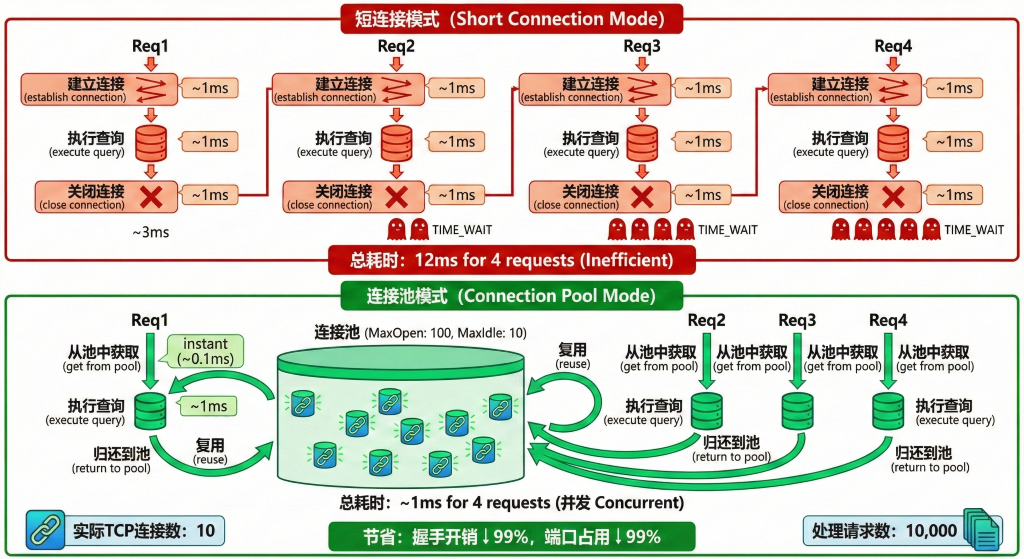
\includegraphics[width=1.0\linewidth]{figures/sec3/image3-6.png}
    \caption{连接池的资源复用机制：通过预创建和重用连接，消除频繁握手和挥手的开销}
    \label{fig:connection-pool}
\end{figure}

连接池的运作机制体现了资源池化管理的核心原则。当业务逻辑发起数据库查询时，连接池首先检查是否有空闲连接可用。如果存在空闲连接，则立即将其标记为占用状态并返回给调用方，整个过程只涉及内存操作，延迟在微秒级别。如果当前没有空闲连接但总连接数未达到上限，连接池会创建新连接并将其加入池中。如果已达到连接数上限，新请求会进入等待队列，直到有其他请求归还连接。当业务逻辑完成数据库操作后，调用连接的关闭方法，但这个"关闭"操作被连接池拦截，实际上只是将连接的状态标记为空闲，重新放入可用队列，而不是真正关闭TCP连接。通过这种"借出-归还"的循环，连接可以被成千上万次地复用，避免了反复握手和挥手的巨大开销。

从云计算的视角看，连接池体现的正是资源池化（Resource Pooling）的核心思想。这是云计算五大特征之一，强调将计算、存储、网络等资源抽象为可动态分配的共享池，按需分配，用完归还，从而最大化资源利用率并降低供给成本。连接池在微观层面实现了这一理念：将稀缺的连接资源组织为共享池，通过精细的生命周期管理实现高效复用。这种池化思想在云原生系统中随处可见，从虚拟机的资源池、容器的镜像缓存池，到负载均衡器的后端服务器池，都是同一设计模式在不同抽象层次的体现。

\subsubsection{对象池：用sync.Pool缓解GC压力}

除了外部连接资源，程序内部的临时对象分配也可能成为性能瓶颈。在游戏服务器的网络层实现中，需要频繁创建和销毁大量临时对象：每次接收网络消息需要分配字节缓冲区（\texttt{[]byte}）用于存储数据，每次解析协议需要创建请求上下文对象，每次序列化响应需要构造JSON编码器，每次日志记录需要分配格式化字符串。这些临时对象的生命周期通常只有几毫秒到几百毫秒，使用完成后立即成为垃圾。在高并发场景下，这些对象的分配和回收频率可能达到每秒数万次甚至数十万次，对Go运行时的垃圾回收器（GC）造成显著压力。

Go的垃圾回收器采用并发标记-清除算法，其设计目标是减少STW（Stop-The-World）暂停时间以保证程序的响应性。但GC并非零成本，每次GC周期仍然需要执行两次短暂的STW暂停：一次在标记开始阶段启用写屏障，一次在标记结束阶段完成最终标记。虽然单次STW时间通常在亚毫秒到几毫秒级别，但在内存分配速率很高的情况下，GC会更频繁地触发，累积的暂停时间会对延迟敏感的应用造成明显影响。对于实时游戏服务器，即使几十毫秒的延迟抖动也可能被玩家感知为卡顿，影响操作的流畅性和战斗判定的准确性。此外，GC在标记阶段需要遍历大量对象的引用关系，这会占用CPU资源并污染处理器缓存，间接降低业务逻辑的执行效率。

\texttt{sync.Pool}提供了一种轻量级的对象复用机制来缓解上述问题。\texttt{sync.Pool}是Go标准库提供的协程安全的对象池实现，专门用于缓存和复用临时对象。其工作原理是维护一个对象缓存，当业务代码需要临时对象时，优先从缓存中获取已有对象；使用完成后，将对象归还到缓存而非立即丢弃。通过这种复用机制，可以显著减少内存分配次数，从而降低GC的触发频率和工作负载。

\begin{tcolorbox}[title=使用sync.Pool复用临时对象]
\begin{lstlisting}[style=codeblock, language=go]
var bufferPool = sync.Pool{
    New: func() interface{} {
        return new(bytes.Buffer)
    },
}

func handleMessage(data []byte) {
    buf := bufferPool.Get().(*bytes.Buffer)
    buf.Reset()
    
    buf.Write(data)
    processData(buf.Bytes())
    
    bufferPool.Put(buf)
}
\end{lstlisting}
\end{tcolorbox}

\texttt{sync.Pool}的使用模式遵循"获取-使用-归还"的三段式流程。\texttt{Get()}方法尝试从池中取出一个对象，如果池中有缓存的对象则直接返回，如果池为空则调用\texttt{New}函数创建新对象。在使用对象之前，务必调用\texttt{Reset()}或类似方法清理对象的状态，确保不会受到之前使用者留下的脏数据影响。业务逻辑使用对象完成工作后，调用\texttt{Put()}方法将对象归还到池中。需要特别注意的是，\texttt{sync.Pool}中的对象不保证一定存在。Go运行时在GC时会清空\texttt{sync.Pool}中的所有对象，这是为了避免池中的对象阻碍GC回收其他内存。因此，\texttt{New}函数是必需的兜底机制，不能假设池中永远有对象可用。

\texttt{sync.Pool}的价值在于打破了"分配-使用-回收"的线性生命周期，将其改造为"分配-使用-缓存-复用"的循环模式。对于那些频繁创建且生命周期很短的对象，复用可以将分配频率从每次请求都分配降低到只在池为空时分配，大幅减少了需要被GC扫描和回收的对象数量。在实践中，合理使用\texttt{sync.Pool}可以将GC暂停时间降低50\%以上，对于追求低延迟的在线服务，这种优化带来的稳定性提升是显著的。然而，\texttt{sync.Pool}并非万能药，它只适合缓存"用完即可丢弃"的短命对象，不适合作为长期持有的状态存储。对于需要跨请求保留状态的数据，应该使用普通的数据结构或专门的缓存系统。

\subsubsection{缓存分层架构：热数据与冷数据的协同治理}

在连接层和内存层完成资源复用优化后，数据访问路径成为影响单机性能的最后一道关口。游戏服务器中的数据访问模式存在显著的频率差异：玩家的实时位置每秒可能更新数十次，在线状态每秒被查询数千次，这些高频数据要求毫秒级甚至亚毫秒级的响应延迟；而账号信息、历史成就、装备配置等数据可能几分钟甚至几小时才被访问一次，但对持久性和一致性有更高要求。如果所有数据都存储在磁盘数据库中，每次查询都需要等待磁盘I/O，在高并发场景下会迅速达到数据库的IOPS上限，导致查询排队和响应延迟恶化。反之，如果所有数据都存储在内存中，虽然访问速度快，但内存成本远高于磁盘，且断电后数据全部丢失，无法满足持久化要求。因此，需要构建分层存储架构，让不同特征的数据存储在最适配的介质上。

\textbf{高频热数据与go-redis}。热数据是指在游戏运行过程中被高频率读取或修改的数据，这类数据对响应延迟极度敏感。典型场景包括玩家在线状态（用于好友系统、组队匹配等功能，每秒可能有数千次查询）、实时游戏状态（MOBA或FPS游戏中的角色坐标、血量、弹药数等战斗数据，更新频率可达每秒数十次）、进行中的对局信息（棋牌游戏的棋盘状态、回合计时器、技能冷却倒计时等临时数据）、实时排行榜（利用Redis的Sorted Set数据结构实现高效的分数排序和范围查询）以及限流计数器（用于防刷机制、API调用频率控制、登录尝试限制等安全功能）。这类数据的共同特征是读写频率高、数据量相对较小、允许短时间的数据丢失（如游戏服务器重启后丢失最近几秒的位置数据是可接受的）。技术策略是将这些数据完全存储在Redis的内存中，通过\texttt{go-redis}客户端进行访问。Redis作为内存数据库，读写延迟通常控制在1毫秒以内，在局域网环境下甚至可以达到亚毫秒级别。\texttt{go-redis}客户端提供了连接池管理、Pipeline批量操作、PubSub消息订阅等高级特性，可以进一步优化访问性能。为了降低数据丢失风险，可以配置Redis的AOF（Append Only File）持久化机制，将写操作记录到磁盘日志，在服务器重启后可以重放日志恢复数据。

\textbf{低频冷数据与gorm + PostgreSQL}。冷数据是指访问频率较低、更新不频繁，但对数据完整性和持久性要求较高的数据。典型场景包括用户注册信息（账号、密码哈希、注册时间、邮箱验证状态等基础身份数据，仅在登录时访问）、历史成就记录（副本通关记录、勋章获取时间、任务完成情况等归档数据，主要用于展示而非实时计算）、基础属性配置（角色初始属性、装备描述文本、技能参数表等静态配置，启动时加载后很少变化）、交易历史（充值记录、道具交易日志、金币流水等需要审计追溯的业务数据）以及全局配置（系统公告内容、活动时间配置、版本兼容信息等运营数据）。这类数据的共同特征是访问频率低、数据量可能很大、必须保证持久性和可恢复性。技术策略是使用\texttt{gorm} ORM框架操作PostgreSQL数据库进行持久化存储。PostgreSQL作为关系型数据库，提供完整的ACID事务语义，可以保证在并发写入、系统崩溃等异常情况下数据的一致性和完整性。\texttt{gorm}简化了SQL操作，提供了模型映射、自动迁移、事务管理等便利功能。冷数据通常在Redis中也会保留一份副本用于加速读取，当Redis中的缓存失效或服务器重启时，可以从PostgreSQL加载权威数据进行恢复。具体的PostgreSQL表结构设计（如玩家账户表、成就记录表、装备配置表）以及对应的gorm模型定义，请参见附录D的实验指南。

\textbf{数据同步策略的选择}。在分层存储架构中，Redis和PostgreSQL之间需要明确的数据同步策略，以保证两层数据的一致性。不同的同步模式在一致性保证、性能开销和适用场景上存在本质差异。写穿（Write Through）模式要求每次写操作同时更新Redis和PostgreSQL，写入操作必须等待两个存储系统都确认成功后才返回。这种模式提供最强的一致性保证，但写入延迟较高，通常在几十毫秒级别。写穿模式适用于数据一致性要求极高的场景，如金币交易、装备绑定、账号状态变更等关键操作，这些操作必须保证Redis和数据库的数据完全同步，避免因不一致导致的经济损失或账号纠纷。写回（Write Back）模式先将数据写入Redis并立即返回，随后通过异步任务定期将Redis中的数据批量刷入PostgreSQL。这种模式的写入延迟低（通常1毫秒内），吞吐量高，但存在数据丢失风险：如果Redis在数据尚未刷入数据库时发生故障，未持久化的数据会永久丢失。写回模式适用于允许短时数据丢失的场景，如玩家位置同步（丢失最近几秒的位置数据可以通过客户端重新上报恢复）、临时状态（如技能冷却时间、战斗Buff等，即使丢失也不影响长期游戏进度）。失效更新（Cache Aside）模式在写入时只更新PostgreSQL，并删除Redis中的对应缓存。下次读取时，发现Redis中没有数据，则从数据库加载并回填到Redis。这种模式适合读多写少的场景，如静态配置数据（物品属性、技能描述、地图配置等）、历史记录查询等。由于配置数据很少变化，大部分读取都能命中Redis缓存，只有在配置更新后的第一次读取会访问数据库。

\begin{figure}[H]
    \centering
    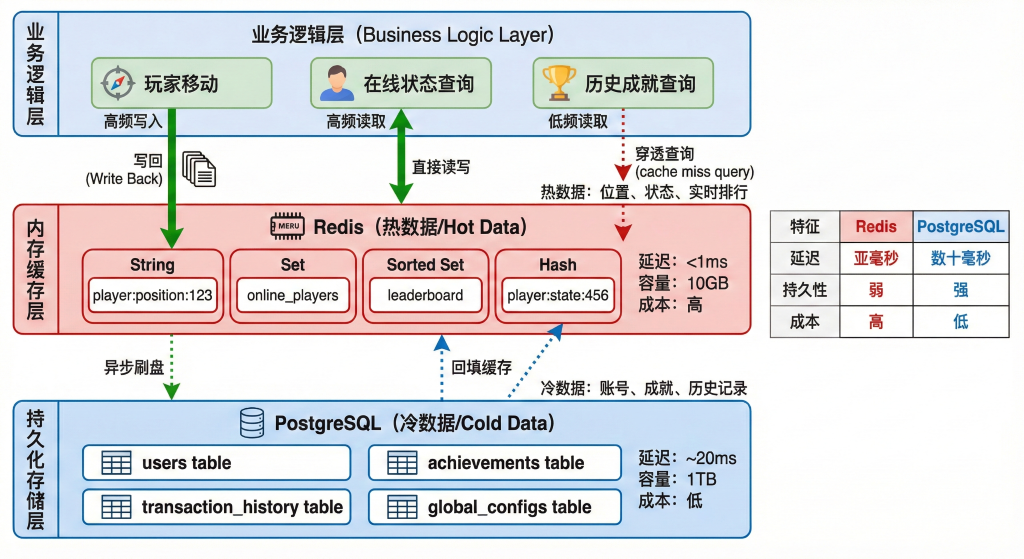
\includegraphics[width=1\linewidth]{figures/sec3/image3-7.png}
    \caption{Redis+PostgreSQL分层存储架构：热数据存内存保证低延迟，冷数据存磁盘保证持久性和低成本}
    \label{fig:redis-postgres}
\end{figure}

表\ref{tab:sync-strategy}总结了三种数据同步策略的特征与适用场景。在实际工程中，不同类型的数据会采用不同的同步策略，以在一致性、性能和成本之间取得最优平衡。

\begin{table}[h]
\centering
\caption{数据同步策略的特征与适用场景}
\label{tab:sync-strategy}
\begin{tabular}{p{3.5cm}p{4cm}p{5cm}}
\hline
\textbf{同步策略} & \textbf{一致性/性能} & \textbf{适用场景} \\
\hline
写穿（Write Through） & 强一致，写延迟高 & 金币交易、装备绑定等关键资产操作 \\
写回（Write Back） & 最终一致，写延迟低 & 玩家位置、临时状态等允许短时丢失的数据 \\
失效更新（Cache Aside） & 最终一致，读性能优 & 物品配置、技能描述等读多写少的静态数据 \\
\hline
\end{tabular}
\end{table}

在实际的游戏服务器中，不同的游戏操作会根据其数据特征选择不同的同步策略。玩家移动是最高频的操作，每秒可能触发数十次坐标更新，但丢失最近几秒的位置数据并不致命——玩家重新连接后客户端会立即上报当前位置，因此移动数据采用写回策略，先写入Redis保证低延迟响应，再由后台任务每隔数秒批量刷入持久存储。击杀与死亡事件虽然频率远低于移动，但它们直接影响排行榜和玩家战绩统计，属于不可丢失的关键事件，因此采用写穿策略，同步写入Redis排行榜和PostgreSQL战绩表，确保两层数据始终一致。金币获取同理——金币是玩家的核心资产，任何丢失都会引发投诉，必须采用写穿策略双写保障。而装备配置、技能参数等静态数据在游戏运行期间几乎不会变化，属于典型的读多写少场景，采用失效更新策略：首次读取时从数据库加载并缓存到Redis，后续读取直接命中缓存；只有在运营人员修改配置时才删除缓存，触发下次读取时重新加载。这种按数据特征选择同步策略的设计思路，是缓存分层架构从理论走向工程落地的关键一步。示例代码中各操作与缓存策略的具体对应关系及实现细节，请参见附录D。

这种分层存储架构不仅是技术实现的优化，更是成本与可靠性的工程权衡。Redis按内存容量计费，成本较高但性能极致；PostgreSQL按存储容量计费，成本低廉但延迟较高。通过将热数据和冷数据分离，可以在满足性能需求的前提下，将存储成本降低数倍。以一个10万在线玩家的游戏为例，如果所有数据都存储在Redis中，每个玩家100KB数据就需要约10GB内存，按云服务商报价计算可能需要数千元月费；而通过分层架构，只将关键热数据（如在线状态、当前位置）存储在Redis中，每玩家仅需1KB，总内存降至100MB，成本降低99\%，而大部分冷数据存储在便宜的PostgreSQL中。这种架构设计体现了云计算"按需使用、成本优化"的核心理念。

\subsubsection{性能验证：用可观测指标量化优化效果}

上述从连接池、对象池到缓存分层的优化设计，本质上都是为了在同一台物理服务器上争取更高的并发承载能力。然而，这些优化是否真正奏效，不能停留在理论分析和直觉判断的层面，而必须通过系统性的压力测试和性能监控来量化验证。只有建立了可观测的性能基线和瓶颈识别能力，才能科学地判断单机优化的边界在哪里，何时应该继续纵向优化，何时必须转向横向扩展。

性能验证的核心在于定义和测量关键指标。对于游戏服务器，最重要的三类指标是吞吐量、延迟分布和资源占用。吞吐量（Throughput）通常用QPS（Queries Per Second）或TPS（Transactions Per Second）来衡量，表示系统每秒能够处理的请求数量。对于我们的游戏服务器，可以测量每秒处理的玩家移动请求数、战斗计算数、状态同步广播数等。吞吐量反映了系统的整体承载能力，是评估优化效果最直观的指标。延迟分布（Latency Distribution）则关注每个请求从发起到收到响应的耗时。与平均延迟相比，P95和P99延迟（即95\%和99\%的请求在多长时间内完成）更能反映用户的真实体验。对于实时游戏，即使平均延迟只有10毫秒，如果P99延迟达到500毫秒，仍然会有1\%的玩家遭遇明显卡顿。资源占用（Resource Utilization）包括CPU使用率、内存占用、网络带宽消耗以及GC统计信息。这些指标帮助我们定位瓶颈所在：如果CPU使用率已达90\%但内存充足，说明瓶颈在计算能力；如果GC暂停频繁，说明内存分配模式需要优化；如果网络带宽打满，说明需要优化消息序列化或引入压缩。

为了量化优化效果，可以设计对比实验。首先，建立基准测试场景：模拟100个并发玩家，每个玩家每秒发送5次移动请求和1次战斗请求，持续运行5分钟，测量未优化版本的性能指标。在这个基准场景下，假设未引入连接池时，由于频繁建连和断连，系统吞吐量可能只有300 QPS，P99延迟达到800毫秒，CPU使用率60\%但大部分时间消耗在系统调用而非业务逻辑。引入数据库连接池后，吞吐量提升到1200 QPS，P99延迟降至150毫秒，因为握手开销大幅减少。进一步引入\texttt{sync.Pool}优化临时对象分配后，GC暂停时间从平均50毫秒降至10毫秒，P99延迟继续降至100毫秒，系统响应更加稳定。最后，引入Redis+PostgreSQL分层架构后，热数据访问延迟从平均20毫秒（访问磁盘数据库）降至1毫秒（访问内存缓存），吞吐量突破2000 QPS，P99延迟稳定在50毫秒以下。通过这样的对比实验，可以清楚地看到每项优化带来的性能提升，也能识别出当前的主要瓶颈。

更重要的是，性能验证帮助我们确定单机优化的边界。当继续增加并发玩家数到500人时，如果发现CPU使用率已达95\%，继续优化代码逻辑只能带来不到5\%的提升，这说明单机的计算能力已接近极限。此时，继续在单机上堆砌优化技巧的收益递减，性价比很低。相反，如果将系统拆分为多个服务实例，通过负载均衡分散请求，可以线性地提升承载能力。这种基于数据的决策判断，正是工程化思维的核心：不是凭感觉优化，而是通过可量化的指标识别瓶颈，评估投入产出比，科学地选择优化方向。当单机优化的边际效益低于横向扩展时，就是转向第四章分布式架构的信号。


\subsection{小结：从“单兵作战”到“军团指挥”}

本章系统性地解决了单机服务器在多人同图场景下的三大核心挑战，完成了从"能运行双人"到"稳定承载多人同图"的关键跨越。在并发组织能力层面，我们通过Goroutine和Channel建立了高效的任务拆解与协作机制，将顺序执行模型改造为可并发的流水线架构。Goroutine的轻量级特性使得"每连接一协程"的架构模式在资源消耗上成为可能，而Channel提供的消息传递机制则将网络I/O层和业务逻辑层有效解耦，使得I/O等待不再阻塞整体吞吐。在正确性保障层面，我们通过Mutex互斥锁机制解决了并发环境下的数据竞争问题，确保关键的游戏规则修改被收敛为原子操作，维护了多人同图场景下规则的确定性和可信度。通过合理设计锁的粒度，在全局锁、区域锁和对象锁之间取得平衡，既保证了正确性又最大化了并发度。在资源效率层面，我们通过连接池复用TCP连接，通过\texttt{sync.Pool}复用临时对象，通过Redis加PostgreSQL的分层架构将数据访问路径优化到极致，在性能、成本和可靠性之间找到了合理的权衡点。

从云计算能力曲线的视角看，本章完成的是纵向优化阶段（Scale Up）的全部任务。我们把单机的并发潜力和资源利用率压榨到了可观测的极限，建立了清晰的性能基线和瓶颈识别能力。通过压力测试和性能监控，我们可以量化地回答：在当前的硬件配置下，单机能够支撑多少并发玩家，每种优化带来了多大的性能提升，以及当前的主要瓶颈在哪里。更重要的是，我们通过性能指标可以科学地判断：当单机CPU使用率已达90\%以上，继续优化代码带来的提升已不足10\%时，纵向优化的边际收益递减，性价比降低。此时，继续在单机上堆砌优化技巧已无法从根本上突破承载能力的天花板，必须转向横向扩展（Scale Out）的分布式架构。

在第四章中，我们将跨越单机边界，进入分布式阶段。此时的核心矛盾将从"如何在单机内高效并发"转变为"如何在多机间保持状态一致"。当游戏世界从单张地图扩展为多张地图、从单个服务实例扩展为多个服务集群时，新的挑战随之而来：跨地图边界的玩家如何感知彼此、跨服战斗的裁决权归属于谁、玩家在不同服务器间迁移时如何保证状态的连续性和一致性。这些问题的本质是分布式系统中的经典难题：数据的跨节点同步、操作的全局顺序保证、以及故障场景下的可用性维护。我们将通过服务拆分、一致性协议和云原生部署等手段，完成从单机优化到分布式协同的架构演进，这正是云计算从"资源可获得"走向"服务可规模化"的关键跨越。




% \subsection{敞开大门：让服务器迎接成千上万的玩家}
% % 具体的实现过程 

% \paragraph{本节目标} 基于 3.1 节确立的技术逻辑框架，围绕 Go 语言并发与高性能网络库优势，探索 “连接池 + 缓存分层” 优化方案，助力突破单机性能瓶颈，提升服务承载能力。
% \paragraph{写作建议}
% \begin{enumerate}
%     \item 基于Go的驱动的优化
%     \paragraph{连接池构建} 基于 3.1 中奠定的技术基础，进一步利用 Go 标准库与sync.Pool，设计协程安全的 TCP 连接池，实现连接复用与生命周期管理。
%     \paragraph{缓存分层架构} 结合go-redis与gorm，分别处理高频与低频数据，在 3.1 逻辑的延伸下，优化读写效率与数据库负载。其中，高频数据指的是在游戏运行过程中被频繁读取或修改的数据，例如玩家当前的游戏在线状态、实时积分、正在进行的游戏对局数据等，这些数据的访问频率极高，将其存储在go-redis缓存中，能快速响应请求，减少数据库压力。而低频数据则是访问频率较低、更新不频繁的数据，像玩家的历史成就记录、注册信息、游戏角色的基础属性配置等，这类数据更适合使用gorm操作pgsql持久化数据库进行存储和管理，既能保证数据的安全性和完整性，又不会因频繁读写影响数据库性能。
%     \item 测量性能。比较单机和并发优化后的单机的承载能力，模拟高并发场景进行压测，监控关键指标并优化系统性能，通过实践验证 3.1 中理论逻辑的实际可行性与优化方向。
% \end{enumerate}



\newpage

% \section*{附录：第三章核心技术索引}

% \newpage